\section{Requirement Gathering and analysis}\label{sec:rga}
Requirement gathering and analysis is the foremost step of SDLC. In this step, we used some requirement gathering techniques like interviews, surveys, and observations. We have partitioned all of the requirements into two separate types which are functional requirements and non-functional requirements.
\subsection{Requirement Gathering}\label{sub:reqgather}
\subsubsection{Functional Requirements:}\label{subsub:funreq}
To collect functional requirements, we meet some teachers from our university and interviewed them. The following are some of their requirements:
\begin{itemize}
	\item Less time-consuming attendance system 
	\item Attendance statistics in detail  should be easy to calculate (From teachers and students ends)
	\item Attendance system must be transparent
	\item Students records should be printable
	\item Less paperwork and one-click procedure
\end{itemize}
Then we meet some administrative officers to meet their requirements and interviewed them. Their requirements include the following things:
\begin{itemize}
	\item Students must be able to enter transaction data into a user interface accepts transaction data.
	\item Students will be able to make fee payments online.
	\item Students should be able to receive feedback on the  online payment.
	\item If the fee payment transaction is successful, students can view, print, or save the payment receipt.
	\item Financial officers will be permitted to lead look on the data of individuals online payment information.
	\item The finance officer will be able to view statistics of all payments made through the system.
	\item Financial officials will provide login information so that  everyone can safely use the system.
	\item Finance officials will be able to see fee payments in an editable manner.
\end{itemize}
Secondly, we conducted a survey among all the students of the University of Chittagong to meet their requirements. According to the survey we have come out with some requirements such as:
\begin{itemize}
	\item Less time-consuming attendance and payment system
	\item Being free from working hours 
	\item Get rid of the tiresome process of queueing
	\item Expanding the ways of transaction
	\item Being independent of a specific bank branch
	\item Being able to make transactions from anywhere
\end{itemize}

\subsubsection{Non-Functional Requirements:}\label{subsub:nonfunreq}
According to the interviews of administrative officers teachers, a survey conducted on students of the University of Chittagong, our observation we find out some non-functional requirements which are as followings:
\begin{itemize}
	\item The system must be easy to operate.
	\item User interface should be simple and understandable for both experienced and inexperienced users.
	\item The system must be secured enough.
	\item Speed of the system should be as fast as possible.
	\item It should be cross-platform compatible.
	\item Reports should be provided in a variety of formats, such as tables and graphs, for simple management visualization.
	\item A standard graphical user interface that facilitates online data entry, modification, update, and deletion.
\end{itemize}
\subsection{Requirement Analysis}\label{sub: reqana}
Post requirement gathering, the step is to analyze it. We have completed this step following the Structured Analysis Methodologies which focuses on the functional decomposition and data-flow analysis. After the brainstorming session of our team members, we come up with a context diagram.\\
\begin{figure}[H]
    \centering
    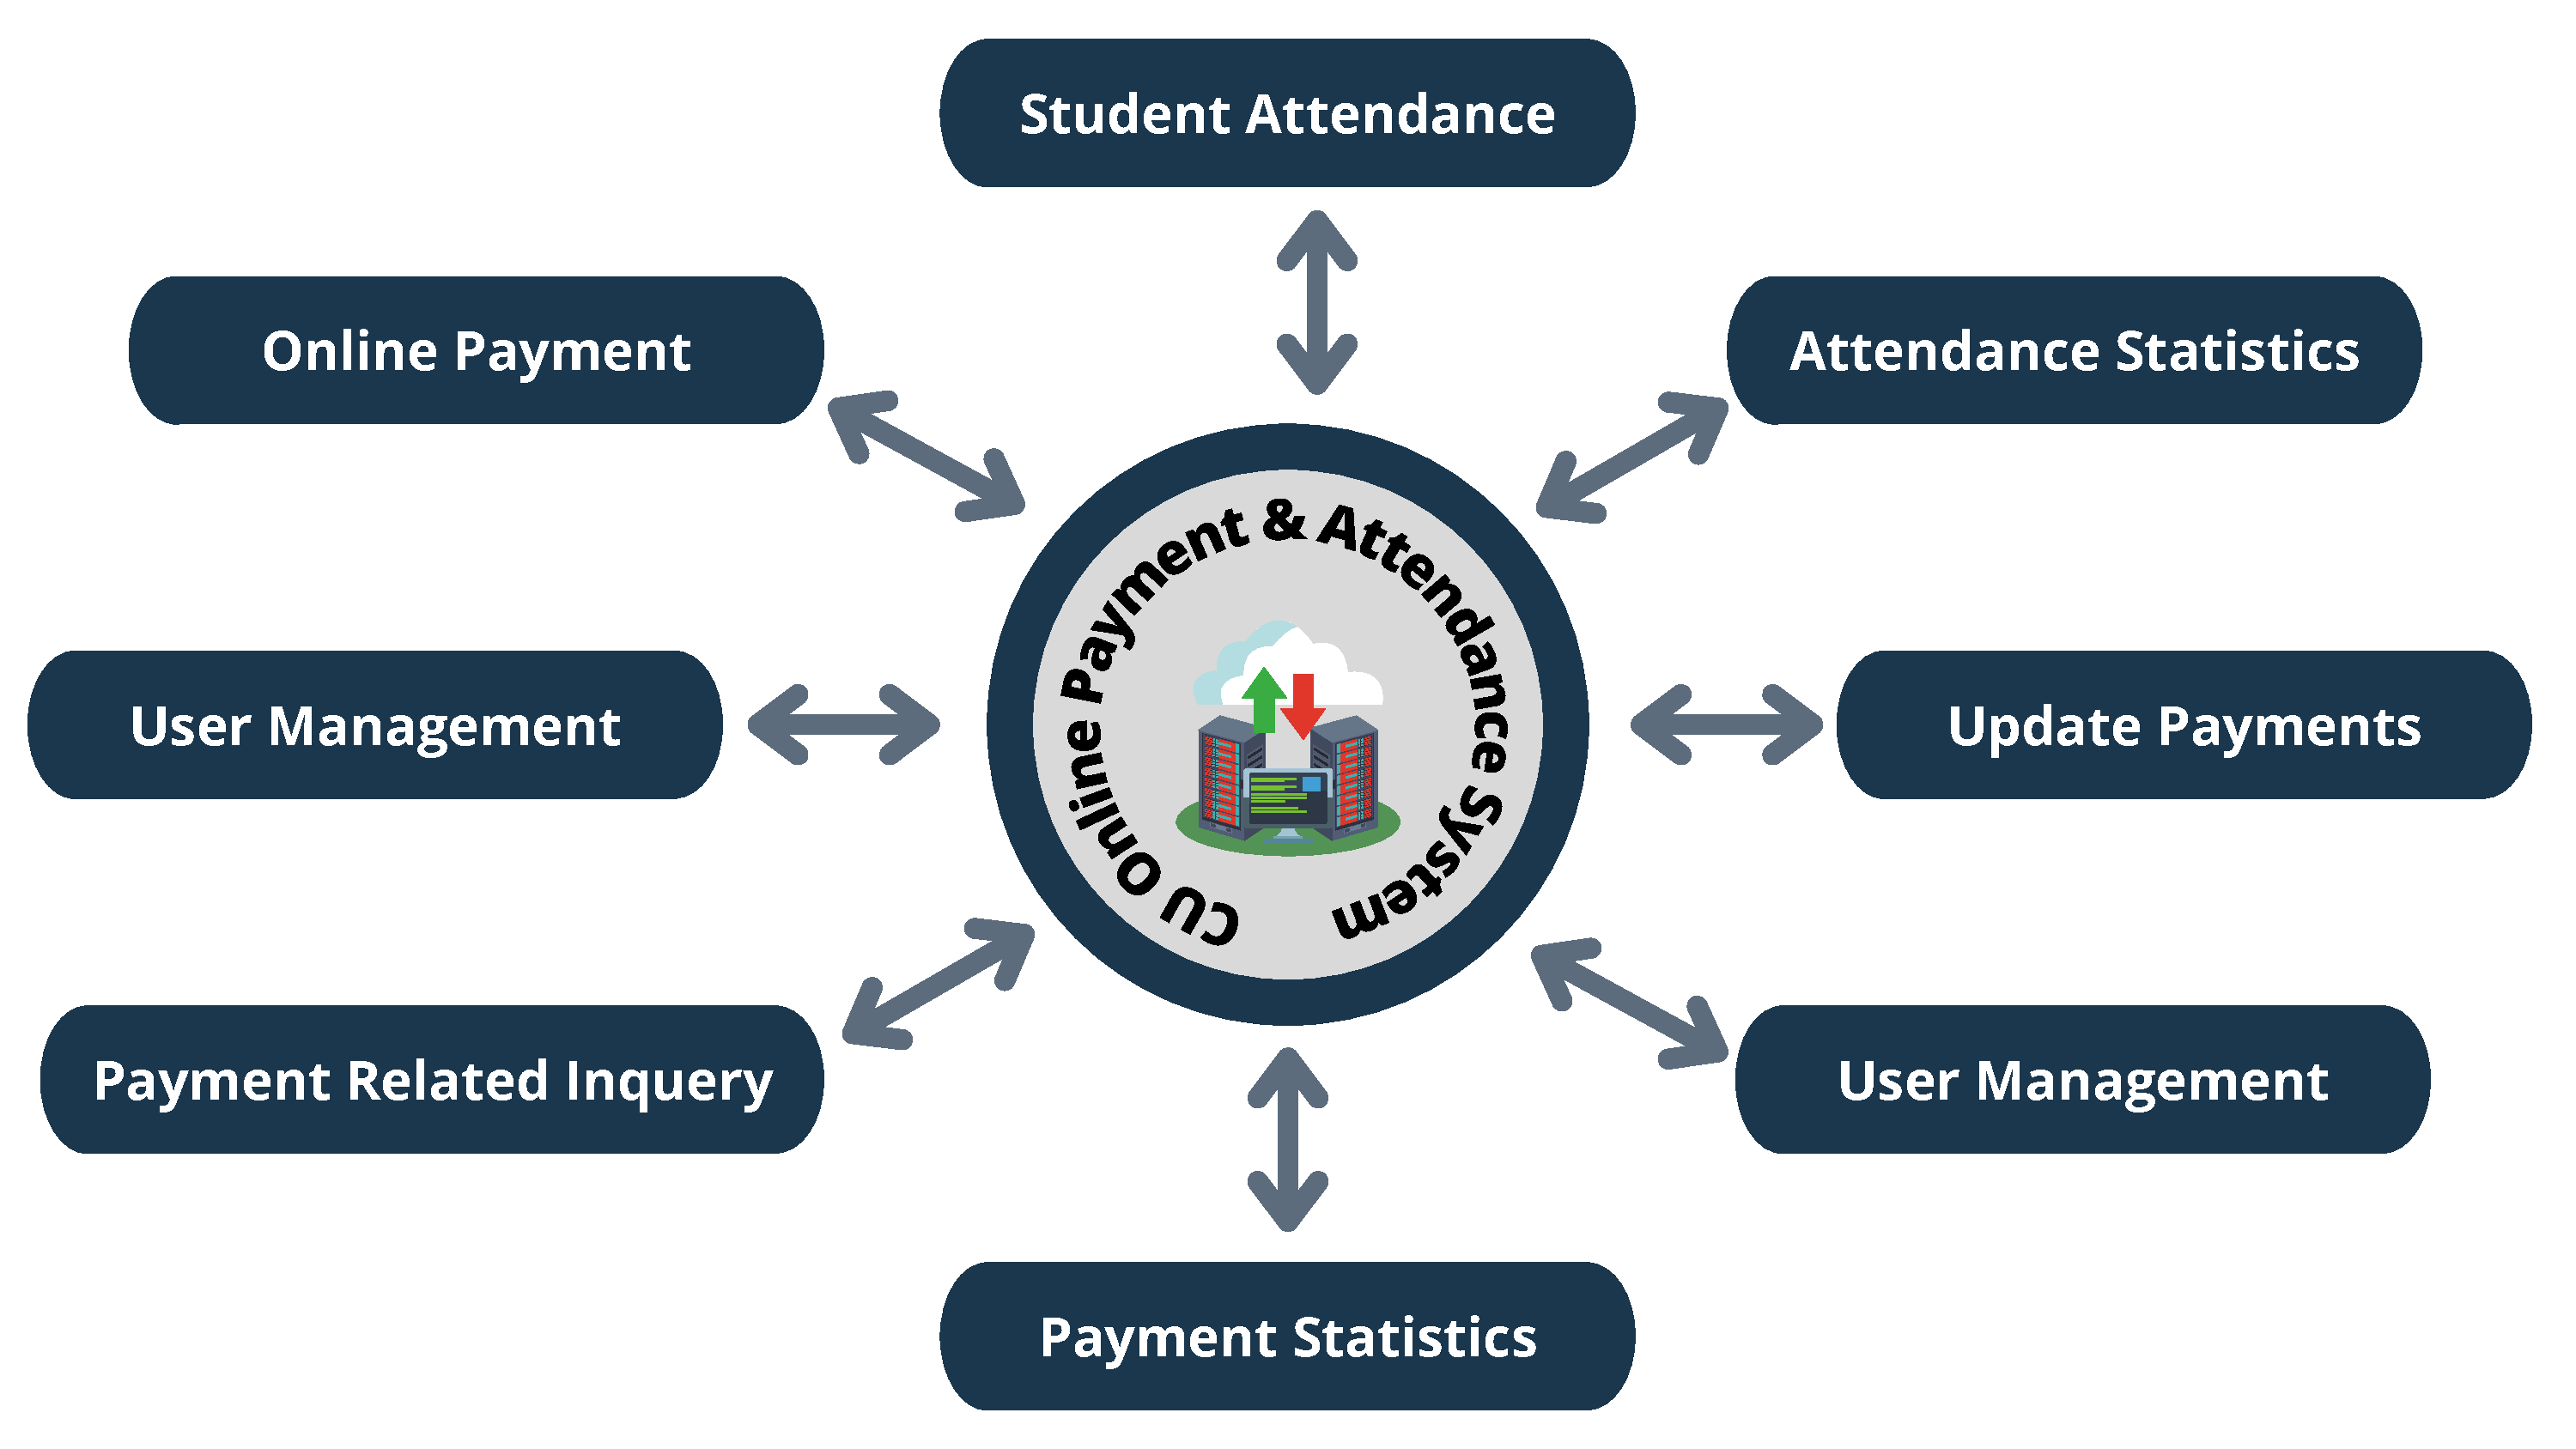
\includegraphics[width=1\textwidth]{images/context}
    \caption{Context Diagram of CU-OPAS}
    \label{fig:context}
\end{figure}
We represented it to the authority as well as our supervisor. Then it was modified a little bit. Finally, we finalized a model of the system which includes all the requirements of administrative officials, teachers, and students which is ready to implement. Then, to define the flow of activities, we created a flowchart.\\
\begin{figure}[H]
    \centering
    \label{fig:flowchart}
    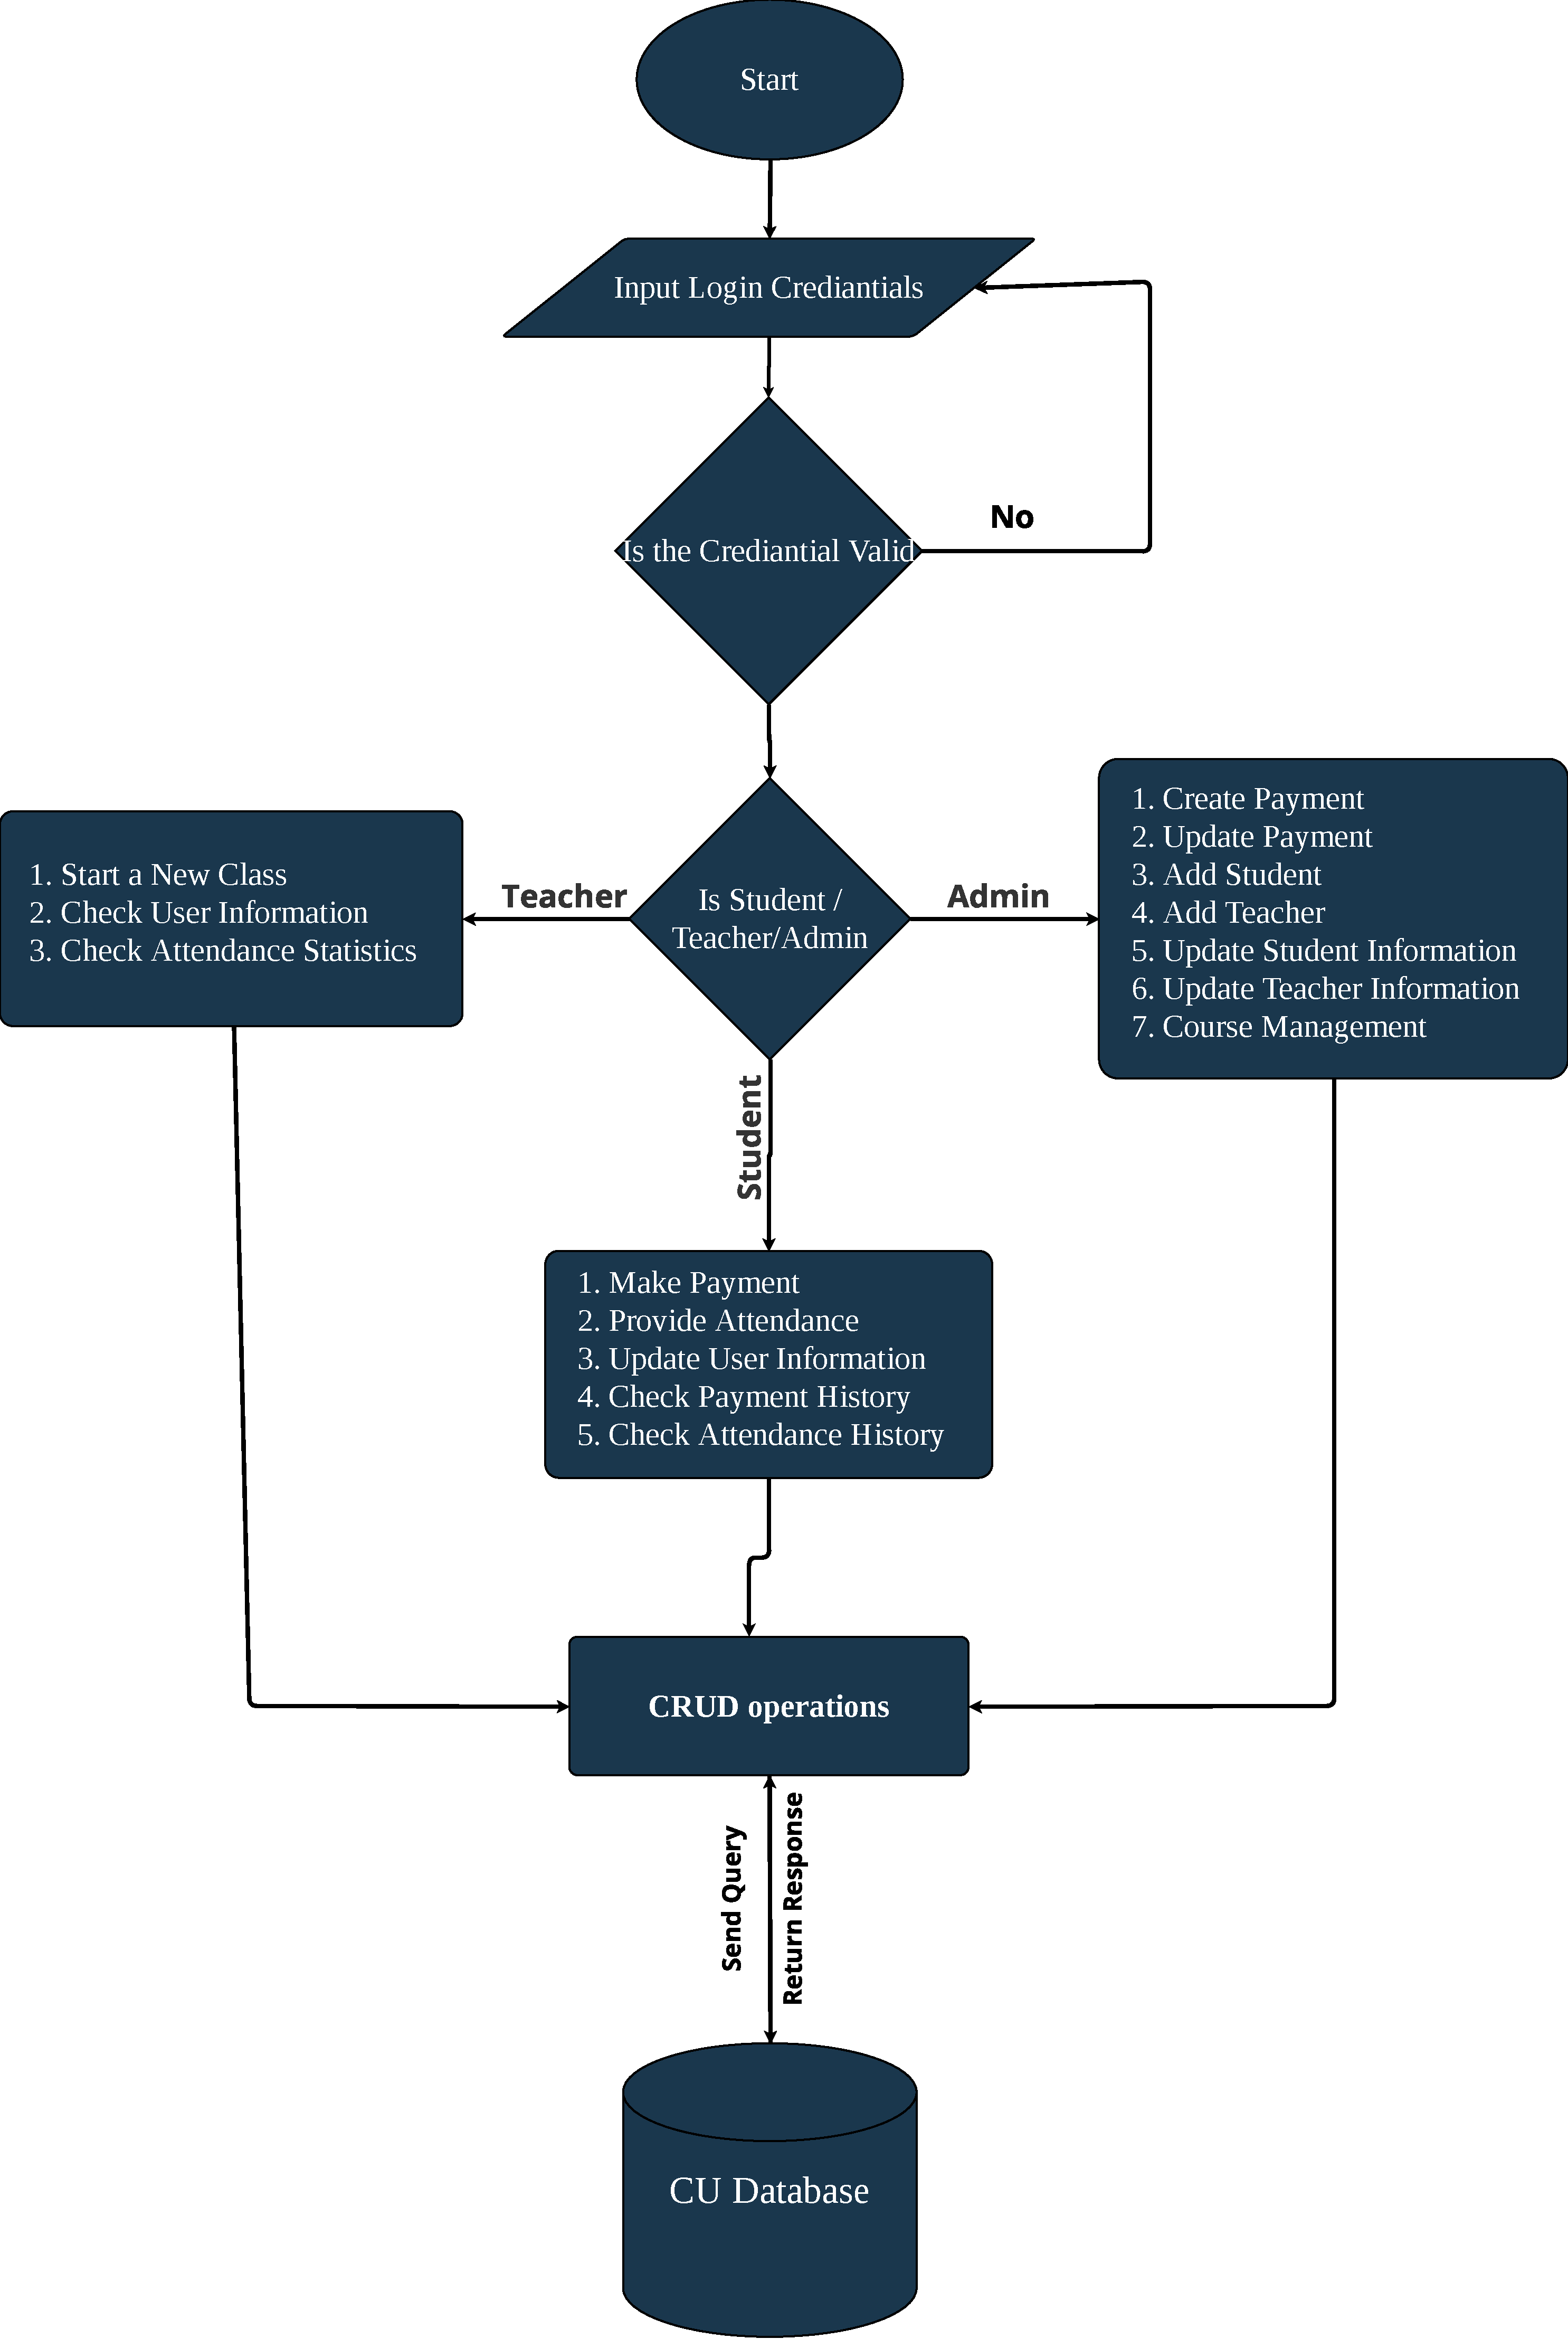
\includegraphics[height=15cm, width=1\textwidth]{images/flowchart}
    \caption{Flowchart of CU-OPAS}
\end{figure}
Finally, we have a completed entity relationship diagram that is ready for implementation.
\begin{figure}[H]
    \centering
    \label{fig:erd}
    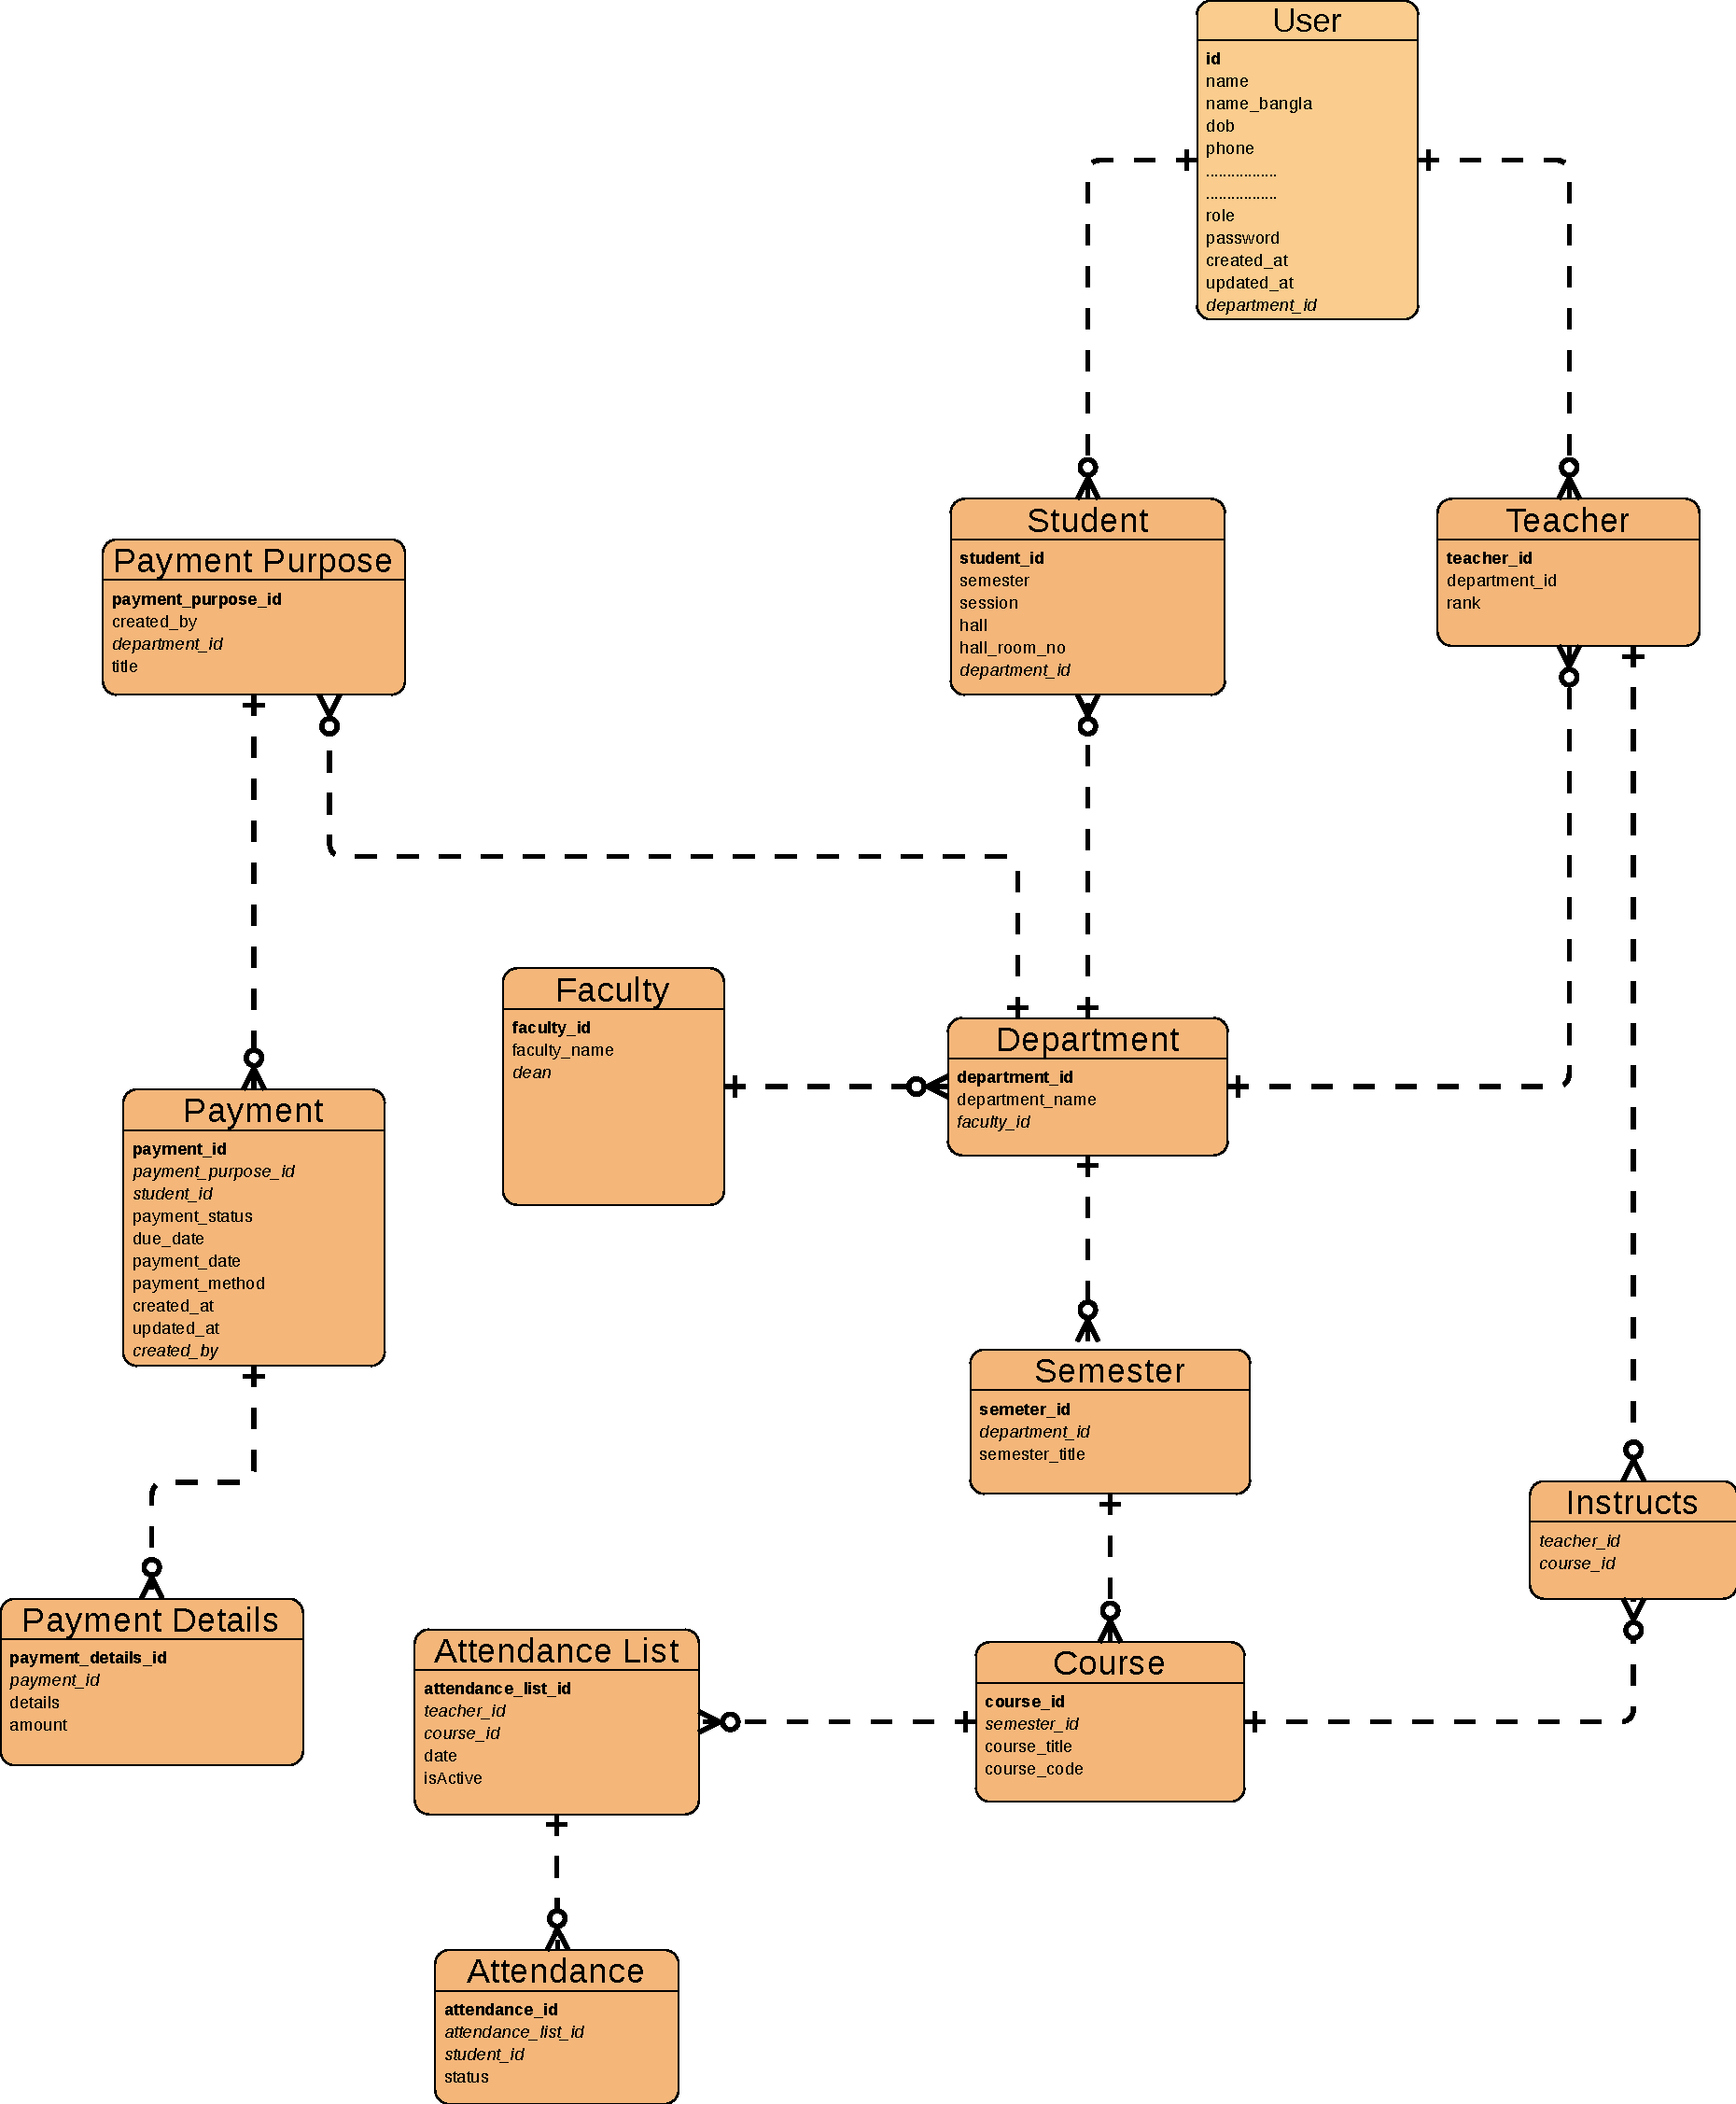
\includegraphics[width=1\textwidth]{images/erd}
    \caption{Entity Relationship Diagram of CU-OPAS}
\end{figure}
Stakeholders are the personnel connected to the project. They are concerned about the outcome of the project. Stakeholders can also be a group, company, customers, suppliers, etc. Stakeholders have a direct or indirect impact on the project. According to this stakeholders are two types i.e. Primary and Secondary. Supervisors, team members, teachers, administrative officials are primary stakeholders, and students, media, other teams including their members are secondary stakeholders in this project.
\clearpage